\documentclass[tikz,border=8pt]{standalone}
% Shared look for every TikZ diagram. Load with \input{../../tools/tikz-style.tex}
\usepackage[T1]{fontenc}
\usepackage{lmodern}
\renewcommand{\sfdefault}{lmr}  % diagrams use the same serif as the text
\usetikzlibrary{arrows.meta, positioning, shapes.geometric, calc, fit, backgrounds}
\definecolor{cblue}{HTML}{4C78A8}
\definecolor{corange}{HTML}{F58518}
\definecolor{cgreen}{HTML}{54A24B}
\definecolor{cred}{HTML}{E45756}
\definecolor{cpurple}{HTML}{B279A2}
\definecolor{cgrey}{HTML}{6B6B6B}
\tikzset{
  every picture/.style={font=\sffamily, line width=1.2pt},
  box/.style={draw=#1, fill=#1!12, rounded corners=4pt, align=center, inner sep=7pt, minimum height=1.1cm},
  box/.default=cgrey,
  arrow/.style={-{Stealth[length=3mm]}, draw=cgrey, line width=1.4pt},
  title/.style={font=\sffamily\bfseries\Large},
  note/.style={font=\sffamily\small, text=cgrey, align=center},
}
\AtBeginDocument{\hyphenpenalty=10000 \exhyphenpenalty=10000}

\begin{document}
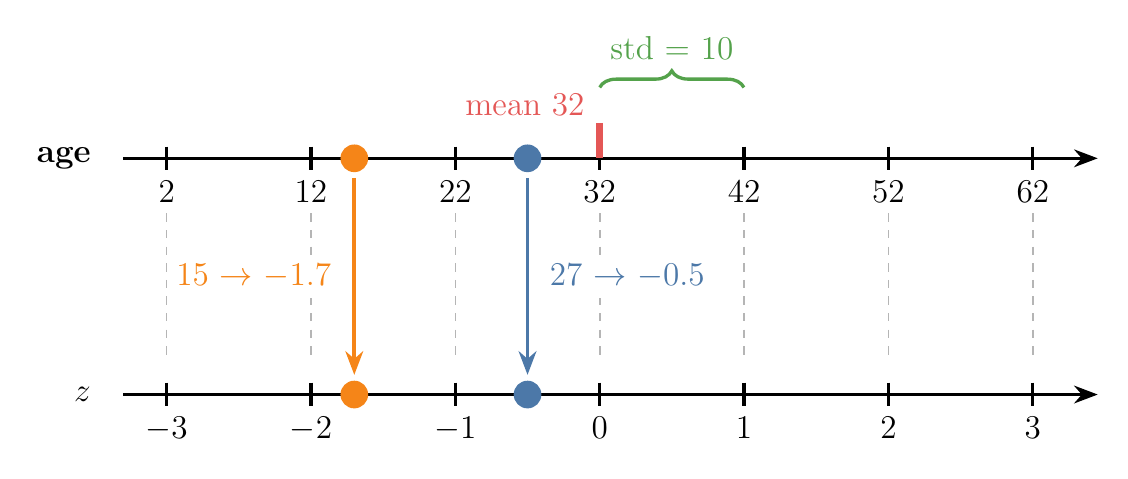
\begin{tikzpicture}[x=0.55cm]
  % top: ages (mean 32, std 10); bottom: the same points in standard deviations
  \node[anchor=east, font=\sffamily\bfseries\large] at (0,0) {age};
  \node[anchor=east, font=\sffamily\bfseries\large] at (0,-3) {$z$};
  \draw[-{Stealth[length=3mm]}] (0.5,0) -- (23,0);
  \draw[-{Stealth[length=3mm]}] (0.5,-3) -- (23,-3);
  \foreach \a/\z in {2/-3,12/-2,22/-1,32/0,42/1,52/2,62/3} {
    \pgfmathsetmacro{\p}{(\a-2)/3+1.5}
    \draw (\p,0.15) -- (\p,-0.15) node[below, font=\large] {\a};
    \draw (\p,-2.85) -- (\p,-3.15) node[below, font=\large] {$\z$};
    \draw[cgrey!50, dashed, line width=0.6pt] (\p,-0.7) -- (\p,-2.5);
  }
  % mean and one std
  \draw[cred, line width=2.5pt] (11.5,0.45) -- (11.5,0);
  \node[cred, anchor=south east, font=\large] at (11.4,0.4) {mean 32};
  \draw[decorate, decoration={brace, amplitude=6pt}, cgreen] (11.5,0.9) -- (14.83,0.9)
    node[midway, above=6pt, font=\large] {std = 10};
  % the two worked customers
  \foreach \a/\z/\c in {27/-0.5/cblue,15/-1.7/corange} {
    \pgfmathsetmacro{\p}{(\a-2)/3+1.5}
    \fill[\c] (\p,0) circle (5pt);
    \fill[\c] (\p,-3) circle (5pt);
    \draw[arrow, draw=\c] (\p,-0.25) -- (\p,-2.75);
  }
  \node[cblue, fill=white, anchor=west, font=\large] at (10.1,-1.5) {27 $\to$ $-0.5$};
  \node[corange, fill=white, anchor=east, font=\large] at (5.55,-1.5) {15 $\to$ $-1.7$};
\end{tikzpicture}
\end{document}
